\section{Approach and Secret Weapon  }

In this project, the data was collected using the public League of Legends API \cite{7_riot_games_2015}.  The raw data was pre-processed after it was collected into suitable formats depending on the machine learning model used.  Further detail is covered in their specific workflows below.

\textbf{Naive Post-match. } Our naive approach analyzed post-match data and tried to analyze whether a 
naive classifier could obtain a higher accuracy given all the information.  
Post-match data contains all the information about the match (except the winning 
team was withheld), including the number of kills on each team, the amount of minions 
that each team kind, the accumulation of gold for each player, etc.  We first pre-process 
the data to create a flattened vector representing the match.  
Given a set of training matches, we can apply the K-Clustering algorithm to train a 
set of \"features\" based on these training matches.  Using Orthogonal Matching Pursuit, we can then create a sparse code representation for these training matches.  
We can then train an SVM classifier using these sparse codes and the 
match outcomes to use for predicting the outcomes of future matches.  
We can test the SVM model by repeating the same process with a new testing data set.  Given that this approach has access to all the post-match data, 
we expect some variables to be highly correlated with the match 
outcome (more kills or more gold probably implies victory).

\textbf{Pre-match. } Our next approach attempts to analyze only the pre-match data in order to create 
a classifier for the match's outcome.  In this case, we only examine variables 
intrinsic to the game itself rather than the performance of the teams and members 
during the match.  An example of an in-game intrinsic is if the team that has a 
certain champion (or set of champions) always seems 
to win or lose.  In this case, we would ignore the statistics of the matches 
actual performance, and instead try to discover whether there are certain inherent 
characteristics of the game that lead to certain advantages.  Our work-flow is similar 
to the one used in the post-game technique.

\begin{figure}[t!]
  \centering
    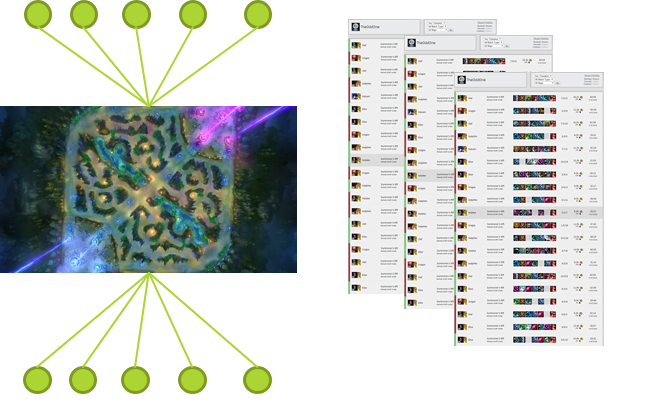
\includegraphics[width=0.5\textwidth]{match+history}
  \caption{Analyzing past match histories grants leverage on identifying meaningful features.  Statistical aggregates are created from a player's recent match history (150 matches). }
  \label{fig:match-history}
\end{figure}

\textbf{Secret Weapon: Match Histories. } Our goal was to be able to predict which team would win a certain match before it occurs. 
We could therefore leverage the knowledge of matches in the past, as well as the pre-game 
information for this certain game.  Our naive post-match method is too constricting, 
requiring us to know the entire post-match data in order to classify the winner.  Our pre-match 
method is not optimal, since it forgoes all the important information that can be extracted 
from past match histories.  Match histories can generate useful information such as 
overall skill level, trends in some of the previously mentioned features, 
affinities for particular champions, and most importantly relationships with other 
players.  Match histories give deeper insight between the possible synergy between 
players that are matched together.  

Analyzing the recent match histories for each of the players in the game 
(five on each team, ten total) would be helpful to build a sophisticated model for the predictor.  
We limit match history calculations to the most recent 150 matches in order to 
minimize data explosion.  Even with this 
limitation, incorporating match histories significantly inflates the amount of 
data required and processed to analyze a single match.  
For example, to process a single match, we now require data from $1 \mbox{ match} * 10 \frac{\mbox{players}}{\mbox{match}} * 150 \frac{\mbox{games}}{\mbox{player}} = 1500 \mbox{ games}$ to be analyzed. 


\textbf{Data Wrangling. } Match histories are most useful when you can determine relationships between the players. 
Single occurences of each relationship would be of little help (i.e., Player 1 and 2 show up on the same or different team only once).
Moreover, the large data explosion that occurs when gathering match history data makes this scenario even less desirable.  However, by carefully selecting the proper subset of matches to analyze, we can increase the overlap of players between matches. League of Legends has a division system (divisions which are called Bronze, Silver, Gold, Platinum, Diamond, Master, and Challenger) which breaks down players based on an ELO-type of rating. The trend seems to show that the higher the division, the less players there are in that division. See Figure \ref{fig:rankedbreakdown} for more details.

\begin{figure}[t!]
  \centering
    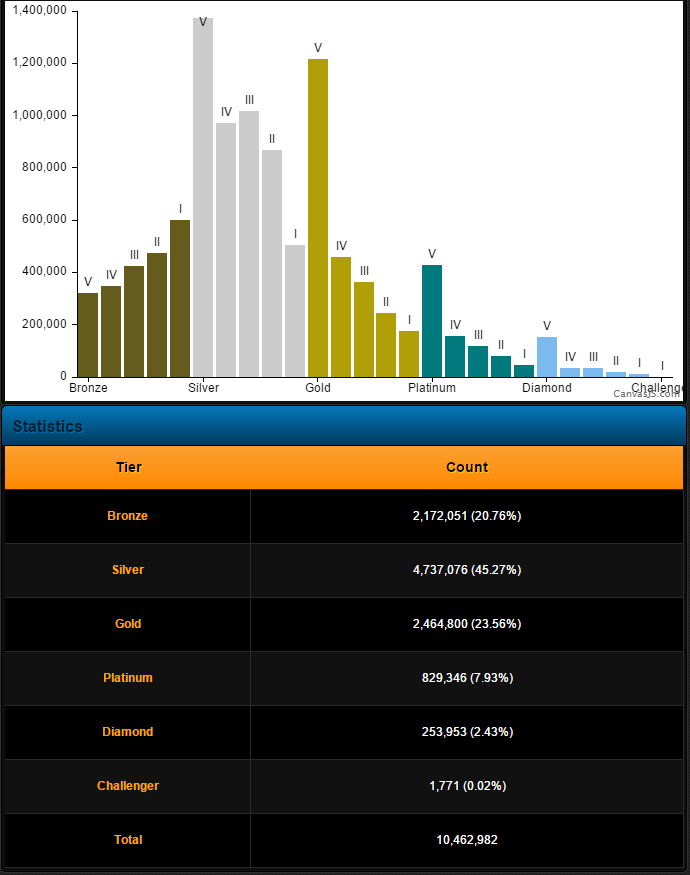
\includegraphics[width=0.5\textwidth]{rankedbreakdown}
  \caption{Higher ranks contain fewer number of players.  This allows us to choose a meaningful subset of players to analyze \cite{8_lolsummoners_2015}. }
  \label{fig:rankedbreakdown}
\end{figure}

Due to this system, people in the higher brackets are matched with the same people much more frequently. We can thus increase the effectiveness of our computation by selecting games of Challenger players. This was seen as in our analysis of 543 games, we archived the history for 787 unique players. This ratio is $\frac{787}{543} = 1.44$ players per game, which is far better than the ratio of 10 unique players per game which we would expect if we looked at a completely random match. 

After acquiring the player histories, the data needs to be pre-processed and converted into a format that can be inputted into an ML model.  As with our previous convention, we want to create a vector (or a matrix in this case, since we have 10 players and multiple features) to represent each match. 

Although applying PCA would be ideal for reducing the dimensions of the data while maintaining variance, we explicitly chose a relatively dense set of features based on 
specific domain knowledge of the game.  The chosen set of features are ("Kills", "Deaths", "Assists", "GoldEarned", "DamageToChampions", "DamageOverall", "GamesPlayed", "Wins"), which should be mostly uncorrelated. This is a good introductory feature set, as though it lacks some of the more complex to express features which mirror complex strategies in the game, it contains the basics.  This step replaces the need to use K-Means clustering to train a feature set. 

Once these features were extracted and transformed into a CSV format easily consumable by the sklearn python module, the data is randomly split into a training and testing set and fed it into a SVM model and a Random Forest Classifier. In this case, no sparsifying of the dataset was done before-hand, as the set of features is expected to be dense.  

\section{System Description. }

The system for the first two techniques has a straight pipeline starting with data pre-processing, to feature extraction, sparse coding, SVM training, and then classification.  This process is described in at a high level in the previous section under Naive Post-match and Pre-match.  This entire process is implemented in Python, using the sklearn library for machine learning.  The sklearn library contains all of the required functionality to do K-Means clustering and SVM classifying.  Many of the components were parallelized using OpenMP for Python.  

\begin{figure}[t!]
  \centering
    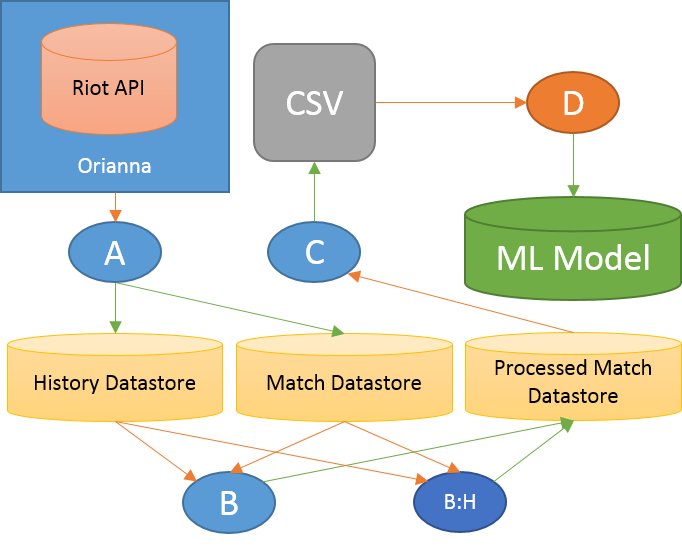
\includegraphics[width=0.5\textwidth]{systemdescription}
  \caption{Steps A, B, C extract features from the data.  Step D creates an ML model.}
  \label{fig:systemdescription}
\end{figure}

We focus our system description on the workflow that models over match histories. Refer to Figure \ref{fig:systemdescription}. 
The first stages (Steps A,B,C) of this process was to extract features from the data and convert this data into a consumable format. This process is described at a high level in the previous section under Data Wrangling.

The data collection stage is done with a Java application using the Orianna project, which wraps the Riot API with a robust interface that among many things allows the retrieved data to be serialized to disk. This step can further be divided into three parts:

\begin{enumerate}
\item Given a player, search through his match history. For every match found iterate through all 10 players and download the match history of each player. This step is very time and disk space expensive, as many many thousands of matches but be written to disk. Also, due to the fact that the Riot API key is rate limited, parallelism is of little use here as the rate limit is the main bottleneck. (This is step A)
\item Given a match, we have 10 players. For each player, iterate through the 150 game history. For each player, create a feature set. In this specific case, we aggregated (summed) certain numeric stats for each player. Align these feature sets so that they are in the form TEAM A:TEAM B:DID TEAM A WIN, where TEAM A = PLAYER 1 STATS:PLAYER 2 STATS: ... : PLAYER 5 STATS and likewise for TEAM B. This is then an array of longs, which is saved to disk. This step is time consuming; in the current Java version multithreading is implemented to accelerate the speed at which matches can be processed. (This is step B)
\item Given a set of matches, convert these into a CSV. This is by far the easiest step, no more than converting a group of serialized long arrays into one CSV. (This is step C)

\end{enumerate}

The second part of the previously detailed process is implemented using Hadoop MapReduce in Java (Step B:H). This allows for much faster processing of matches in parallel. However, it is very memory intensive (thousands of matches must be loaded into memory for analysis) so depending of hardware constraints 
the Java multi-threaded version could be faster/more optimal to use. 

The second stage (Step D) of this project is to once data has been aggregated, to consume this data and produce a model, and to see how accurate this model is. As stated earlier, sklearn was used, specifically SVM and Random Decision Forests. This train and test models using cross validation if opted for, and to save the model to disk if opted for. 

\begin{figure}[t!]
  \centering
    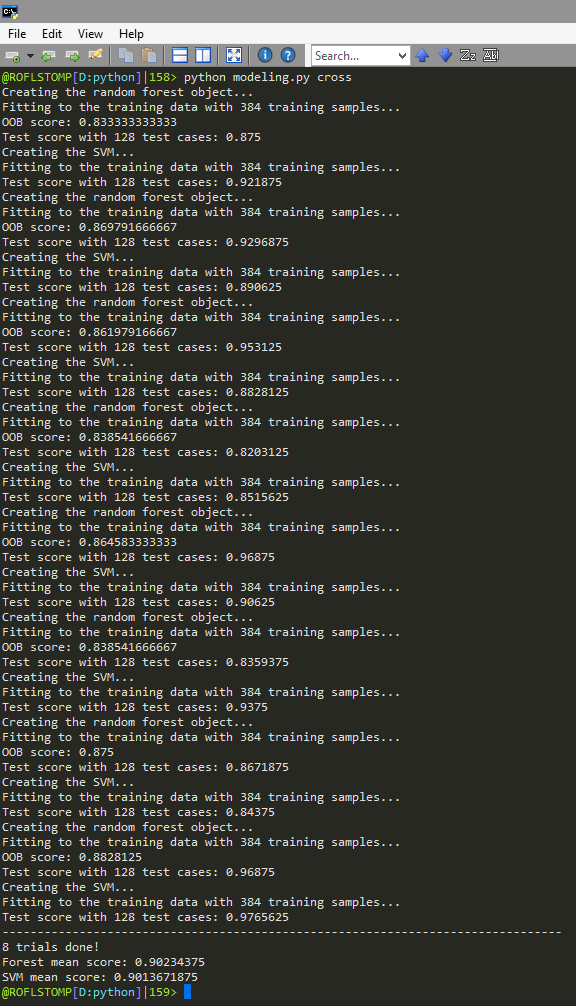
\includegraphics[width=0.5\textwidth]{modelscore}
  \caption{Output of match history model.}
  \label{fig:modelscore}
\end{figure}

\section{Performance Evaluation}
\textbf{Speed. } In all of the workflows above, the data collection and pre-processing took the bulk of the time.  We focus on the description of our main sophisticated system, but the results are very similar in our first two workflows.  Our data collection is limited by the API-rate allowed by the developers of League of Legends.  As of now, there is no real way to get around the API limit without obtaining a 
production key or exploiting multiple API keys. Step 1 took over 100 compute hours to aggregate the 512 datapoints into the final data format.

\textbf{Accuracy. } The first naive model produced results in the upper 90\%, as expected given the abundance of information given as inputs.  Our analysis seemed to indicate that given the post-match data, there are very clear and strong correlations between certain statistics and the game's outcome.  This knowledge later motivated the specifically chosen feature set in the match-history model.

The second model that predicts using only pre-match information produced accuracy rates of around 60-65\%.  These results seem to imply that there are certain traits and characteristics that are inherent to the game that make certain team match-ups better than others.  However, the lack of accuracy results from the discarding of large amounts of data related to post-game results.  

The final model hovers at around 90\% accuracy over 384 test and 128 train datapoints. These results are produced from randomly segregations into those splits given an initial 512-sample set. This is surprisingly high given the small data set.  However, there may be issues of over-fitting given the relatively small sample size.
